\documentclass[journal,10pt]{IEEEtran}
\usepackage{amsmath,epsfig,amssymb}
\usepackage{color}
\usepackage{amsfonts,bm,subfigure,cite}
%\usepackage{geometry}
%\geometry{a4paper,scale=0.8}
%\geometry{bottom=1cm}
% \usepackage[top=1in, bottom=1in, left=1in, right=1in]{geometry}
% \usepackage[top=0.8in, bottom=0.4in, left=0.5in, right=0.5in]{geometry}
\usepackage{balance}

\def \blkdiag{\operatorname{blkdiag}}
\def \diag{\operatorname{diag}}
\def \ln{\operatorname{ln}}
\def \arg{\operatorname{arg}}
\def \tr{\operatorname{tr}}

\begin{document}

\title{Blind Direct Position Determination Of Multiple Frequency Hopped Signals}

\author{Kegang~Hao,~\IEEEmembership{Student Member,~IEEE,}
        and~Qun~Wan,~\IEEEmembership{Member,~IEEE}
        
\thanks{This work was supported in part by the National Natural Science Foundation of China (NSFC) under Grant 61771108 and U1533125, and the Fundamental Research Funds for the Central Universities under Grant ZYGX2015Z011.

    K.G. Hao and Q. Wan are with the University of Electronic Science and Technology of China, Chengdu 611731, China, (e-mail:haokegang@std.uestc.edu.cn).}
}

\maketitle

\begin{abstract}
The common approach to solve the blind multiple frequency hopped (FH) signals localization problem is AOA (Angle Of Arrival) based methods because
they don't require estimating the FH pattern to identify the idle frequencies since the data model is built in space domain.
However, in multiple emitters scenario, the AOA based methods have limited accuracy and resolution since they are sensitive to the unmodeled dynamics (i.e. frequency hopping).
In order to improve the performance of localizing multiple FH signals, we don't only model the location information in space domain but also in frequency domain.
The more complex model means more unknown parameters to estimate. In order to avoid multidimensional searching, 
we propose a MUSIC (MUltiple SIgnal Classification) based algorithm to Determinate emitter Positions Directly (DPD) from the received data, meanwhile, the idle frequencies are identified and the corresponding noise is removed. 
The simulation results indicate that the proposed estimator outperforms the AOA based estimator both in the aspects of accuracy and resolution and attains asymptotic optimal performance.  
\end{abstract}

\begin{IEEEkeywords}
frequency hopping Sequence estimation, Direct Position Determination, MUltiple SIgnal Classification (MUSIC) 
\end{IEEEkeywords}


\IEEEpeerreviewmaketitle


\section{Introduction}
\label{sec:intro}

\IEEEPARstart{F}{requency} Hopped Code-Division Multiple Access (FH-CDMA) is an appealing spread spectrum technique in wireless communication 
because FH provides resistance to multiple-access interference without requiring stringent power control to alleviate the near-far problem, 
as required for direct-sequence CDMA \cite{torrieri2000mobile}.
Frequency-hopped spread spectrum (FHSS) has been adopted in two commercial standards: IEEE 802.11 (Wireless LAN) and Bluetooth
(Wireless PAN) which are very common in our life. It is also the prevailing spread-spectrum technique in military communications \cite{torrieri1997future}, 
largely due to its robustness to jamming coupled with low probability of intercept/ detection (LPI/LPD) and good near–far properties.

As the FHSS has been applied widely in military and commercial communication systems,
the demand for blind localization of FH emitters, such as localization of the illegal Unmanned Aerial Vehicle (UAV) nearby airport 
or the interception of noncooperative military communications, increases rapidly, which has attracted much interests on the localization technique for FH signals\cite{liu2002blind,liu2010ziv–zakai}.

On the technical side, the blind localization problem is challenging not only because both of FH sequences and the emitter locations are unknown but the hop-timing is also unknown. 
The method proposed in \cite{liu2002blind} exactly needs a preprocessing step to detect the hop-timing in the received data stream so that
the hop-free data subset can be identified and used to estimate the AOA. While the AOA estimator is sensitive to the unmodeled dynamics 
which are introduced in by the imperfect hop-timing detection\cite{liu2002blind}. In the view of information theory, the additional preprocessing steps (including hop-timing detection and estimating DOAs) are likely to result in more loss of information about emitter locations. 
% The method proposed in \cite{liu2002blind} also makes an important assumption that the array steering vectors are quasi-stationary,
% which means the range of FH satisfies the narrowband assumption. While carrier FH is very common in realistic scenario, the range of which can be very wide.
% In such realistic situation, the array steering vectors are no longer quasi-stationary, due to wavelength-dependent phase shifting from one array element to another. 

The DPD approaches \cite{Weiss2004Direct,Weiss2011Direct,HighResolutionKG} have recently attracted much interests for its outstanding performance at low Signal to Noise Ratio (SNR) ,compared with the traditional two-step approach. 
The DPD approach estimates the parameters of interest by minimizing a single cost function into which all received data batches enter jointly.
However, the Time Difference of Arrival (TDOA) based DPD method for multiple FH emitters proposed in \cite{ouyang2017direct} assumes FH sequence as a prior knowledge, which is impractical in noncooperative scenario.
From the view of information theory, the traditional two-step approach is more likely to damage the position information during the estimation of intermediate parameters that DPD approach avoids.
Thus, we tend to build the parameterized data model of the received signals based on the emitter locations and FH sequences directly.

In this paper, we build a data model to describe the location information of multiple FH emitters both in space and frequency domain. 
Based on the space-frequency data model, the emitter locations and FH sequences are estimated jointly without the prior knowledge of FH patterns.
The received data from all sensors are collected to identify the idle frequencies while only data from the reference sensor are used by the estimator in \cite{liu2002blind}.
On the other hand, the location information in frequency domain is exploited to improve the localization performance. 

\section{Problem formulation}
\label{sec:model}

\subsection{the received FH signal model}
Considering $N_r$ receivers whose positions are denoted by the vectors of coordinates 
$\boldsymbol{r}_j,j=1,\dots,N_r$ and each receiver is equipped with an array of $M$ elements. $Q$ FH emitters are located at $\boldsymbol{p}_q,q=1,\dots,Q$. The envelope of $q$-th FH signal is given by
\begin{align}\label{eq:1}
    u_q(t)=\sum_{h=1}^H u_{q,h}(t-(h-1)T_d)
\end{align} 
where $H$ is the number of hopping, $T_d$ is the duration time of each hopping and $u_{q,h}(t)$ is the $h$-th hopped signal envelope.

The complex envelope of the signals intercepted by the $j$-th receiver is given as
\begin{align}\label{eq:2}
    \boldsymbol{s}_j(t)= \sum_{q=1}^{Q}\mu_{j,q} \boldsymbol{a}_j(\boldsymbol{p}_q)u_q(t-\tau_j(\boldsymbol{p}_q))+\boldsymbol{n}_j(t) \quad t\in [0,T]  
\end{align}
where $\mu_{j,q} $ is an unknown complex scalar representing the signal attenuation due to path loss between 
the $j$-th receiver and the $q$-th emitter. $u_q(t-\tau_j(\boldsymbol{p}_q))$ is the $q$-th transmitted signal delayed by $\tau_j(\boldsymbol{p}_q)\triangleq\Vert\boldsymbol{r}_j-\boldsymbol{p}_q\Vert/c$, $c$ is the light velocity.
$\boldsymbol{n}_j(t)$ represents zero-mean, white, circular complex Gaussian noise whose covariance matrix is $\sigma^2\boldsymbol{I}_M$. %($\boldsymbol{I}_M$ is identity matrix).
%Taking the carrier hopping into account, the narrowband assumption no longer holds, so that the spatial steering vector relies on the hopping frequency $f_h$,
The steering vector 
\begin{align}\label{eq:3}
    \boldsymbol{a}_j(\boldsymbol{p}_q)&\triangleq [1 \quad \dots \quad e^{j\boldsymbol{k}^T_j(\boldsymbol{p}_q)\boldsymbol{d}_M}]^T
\end{align} 
where 
\begin{align}\label{eq:4}
    \boldsymbol{k}_j(\boldsymbol{p}_q)\triangleq \frac{2\pi f_c(\boldsymbol{r}_j-\boldsymbol{p}_q) }{c\Vert\boldsymbol{r}_j-\boldsymbol{p}_q \Vert} 
\end{align} 
$\boldsymbol{d}_m$ denotes the location of the $m$-th array element relative to that of the reference array element.

The observed signal time interval $[0,T]$ can be partitioned into $L$ sections, each of length $T/L$. Sampling the received signal \eqref{eq:2} by period $T_s$ in every section, the discrete sample data are given as,
\begin{align}\label{eq:5}
    \boldsymbol{s}_j(nT_s,l)=\sum_{q=1}^{Q} \mu_{j,q} \boldsymbol{a}_j(\boldsymbol{p}_q)u_q(nT_s-\tau_j(\boldsymbol{p}_q),l)+\boldsymbol{n}_j(nT_s,l)
\end{align}
where $l=1,\dots,L$ are the batch indexes and $n=1,\dots,N$ are the sample indexes of each batch. It is assumed that $\max_j \tau_j(\boldsymbol{p}_q)\ll T/L$, which can be obtained by using long enough observation interval for 
the region of interest. 

\subsection{frequency hopping/non-hopping sequences}
During each observation section, We sample total $K$ frequency points in frequency band of interest. For the $K$ frequency points, $2^K$ possible frequency hopping/non-hopping sequence per FH signal can be formed.
The $\kappa$-th possible sequence reads $S_{q,\kappa}=(b_q(1),\dots, b_q(K))_\kappa,\kappa=1,\dots,2^K$, where $b_q(k)$ is a binary variable that corresponds to the case 
where the $q$-th FH signal has hopped to the $k$-th frequency. For the given $q$-th FH pattern, it is assumed that the probability of hopping to the $k$-th frequency $P(b_q(k)=1)=P_{q,k}$ is constant.
The probability of occurrence of a particular frequency hopping/non-hopping sequence is given by
\begin{align}\label{eq:6}
    P(S_{q,\kappa})=\prod_{k\in K_\kappa}P_{q,k}\prod_{\bar{k}\in \bar{K}_\kappa}(1-P_{q,\bar{k}})
\end{align}
where $K_\kappa$ and $\bar{K}_\kappa$ are the number of frequency points where the $q$-th FH signal does hop to and does not hop to, respectively.

We call the collection for the sequences of all FH signals an event. For $Q$ FH signals, $2^{KQ}$ collections of independent frequency hopping/non-hopping sequences are the possible events.
The probability of occurrence of a particular event $E_{\kappa_1\dots\kappa_Q}=(S_{1,\kappa_1},\dots,S_{Q,\kappa_Q})^T$, is given by 
\begin{align}\label{eq:7}
    P(E_{\kappa_1\dots\kappa_Q})=\prod_{q=1}^Q P(S_{q,\kappa_q})
\end{align}
Given a particular event $E_{\kappa_1\dots\kappa_Q}$, the effective number of FH signals at $k$-th frequency point is given as $Q_k=\sum_{q=1}^Q b_q(k)$. 
It can be seen that only a part of FH signals ($Q_k<Q$) are observed at every frequency point and each FH signal tends to occur at frequency points with high probabilities $P_{q,k}$.
Thus, in order to localize the $q$-th FH signal accurately, we need to identify the idle frequency points of the $q$-th FH signal ($b_q(k)=0$) and remove the noise at these frequency points.

\subsection{data model}
In order to extract the position information from the transmitted waveform $u_q(nT_s-\tau_j(\boldsymbol{p}_q),l)$, 
each section of received signal \eqref{eq:5} need to be represented in frequency domain by the Discrete Fourier Transformation (DFT), 
\begin{align}\label{eq:8}
    \bar{\boldsymbol{s}}_j(k,l)=\sum_{q=1}^Q  \mu_{j,q}\bar{\boldsymbol{a}}_j(k,\boldsymbol{p}_q) b_q(k,l)\bar{u}_q(k,l)+\bar{\boldsymbol{n}}_j(k,l)
\end{align}
where 
\begin{align}\label{eq:9}
    \bar{\boldsymbol{a}}_j(k,\boldsymbol{p}_q)\triangleq \boldsymbol{a}_j(\boldsymbol{p}_q)e^{-j2\pi k\tau_j(\boldsymbol{p}_q)/(NT_s)}
\end{align}
contains all information about emitter positions.
$k=1,\dots,K$ are the indexes of Fourier coefficients. $b_q(k,l)$ is the sample of random variable $b_q(k)$, which is a binary variable that corresponds to the case 
where the $q$-th FH signal has hopped to the $k$-th frequency during the $l$-th observation section. 
$\bar{u}_q(k,l)$ and $\bar{\boldsymbol{n}}_j(k,l)$ are the DFT of the transmitted signal and noise respectively.

By stacking the sample vectors in \eqref{eq:6} along the index $j$, we get
\begin{align}\label{eq:10}
    \bar{\boldsymbol{s}}(k,l)=\sum_{q=1}^Q \bar{\boldsymbol{a}}(k,\boldsymbol{p}_q,\boldsymbol{\mu}_{q}) \tilde{u}_q(k,l) +\bar{\boldsymbol{n}}(k,l)
\end{align}
where 
\begin{align*}
    \bar{\boldsymbol{s}}(k,l)&\triangleq[\bar{\boldsymbol{s}}_1^T(k,l)\quad  \cdots \quad \bar{\boldsymbol{s}}_{N_r}^T(k,l)]^T &\in \mathbb{C}^{N_rM }\\
    \bar{\boldsymbol{a}}(k,\boldsymbol{p}_q,\boldsymbol{\mu}_{q})&=\left[
     \begin{array}{c}
        \mu_{1,q}\bar{\boldsymbol{a}}_1(k,\boldsymbol{p}_q)\\
        \vdots\\
        \mu_{N_r,q}\bar{\boldsymbol{a}}_{N_r}(k,\boldsymbol{p}_q)
     \end{array}
        \right]&\in \mathbb{C}^{N_rM\times 1}\\
    \boldsymbol{\mu}_{q}&=[\mu_{1,q} \quad \cdots \quad \mu_{N_r,q}]^T &\in \mathbb{C}^{N_r\times 1} \\ 
    \tilde{u}_q(k,l)&=b_q(k,l)\bar{u}_q(k,l)&\in \mathbb{C}\\
    \bar{\boldsymbol{n}}(k,l)&=[\bar{\boldsymbol{n}}_1^T(k,l)\quad \cdots \quad \bar{\boldsymbol{n}}_{N_r}^T(k,l)]^T &\in \mathbb{C}^{N_rM}
\end{align*}

And then, the matrix form of \eqref{eq:8} is given as,
\begin{align}\label{eq:11}
    \bar{\boldsymbol{s}}(k,l)= \bar{\boldsymbol{A}}_k(\boldsymbol{\xi},\boldsymbol{\theta}) \cdot \tilde{\boldsymbol{u}}(k,l)+\bar{\boldsymbol{n}}(k,l)
\end{align}
where
\begin{align*}  
    \boldsymbol{\xi}&=\{\boldsymbol{p}_1, \dots ,\boldsymbol{p}_Q\},\quad 
    \boldsymbol{\theta}=\{\boldsymbol{\mu}_{1},\dots ,\boldsymbol{\mu}_{Q}\}\\
    \bar{\boldsymbol{A}}_k(\boldsymbol{\xi},\boldsymbol{\theta})&=[\bar{\boldsymbol{a}}(k,\boldsymbol{p}_1,\boldsymbol{\mu}_{1})\quad \cdots \quad \bar{\boldsymbol{a}}(k,\boldsymbol{p}_Q,\boldsymbol{\mu}_{Q})] &\in \mathbb{C}^{N_rM\times Q}\\   
    \tilde{\boldsymbol{u}}(k,l)&=[\tilde{u}_1(k,l) \quad \cdots \quad \tilde{u}_Q(k,l)]^T &\in \mathbb{C}^{Q\times 1}  
\end{align*}
Keep stacking the signal model along the index $k$, the compact signal model can be written as,
\begin{align}\label{eq:12}
    \bar{\boldsymbol{s}}(l)=\tilde{\boldsymbol{A}}(\boldsymbol{\xi},\boldsymbol{\theta})\tilde{\boldsymbol{u}}(l)+\bar{\boldsymbol{n}}(l) 
\end{align}
where 
\begin{align*}
    \bar{\boldsymbol{s}}(l)&\triangleq[\bar{\boldsymbol{s}}^T(1,l)\quad  \cdots \quad \bar{\boldsymbol{s}}^T(K,l)]^T \in \mathbb{C}^{KN_rM\times 1 }\\
    \tilde{\boldsymbol{A}}(\boldsymbol{\xi},\boldsymbol{\theta})&=\diag \{\bar{\boldsymbol{A}}_1(\boldsymbol{\xi},\boldsymbol{\theta}),\dots,\bar{\boldsymbol{A}}_K(\boldsymbol{\xi},\boldsymbol{\theta})\} \in \mathbb{C}^{KN_rM\times KQ}\\
    \tilde{\boldsymbol{u}}(l)&=[\tilde{\boldsymbol{u}}^T(1,l) \quad \cdots \quad \tilde{\boldsymbol{u}}^T(K,l)]^T \in \mathbb{C}^{KQ\times 1}\\
    \bar{\boldsymbol{n}}(l)&=[\bar{\boldsymbol{n}}^T(1,l)\quad \cdots \quad \bar{\boldsymbol{n}}^T(K,l)]^T\in \mathbb{C}^{KN_rM\times 1 }
\end{align*}
It can be seen that all information about emitter locations is embedded in the array manifold  $\tilde{\boldsymbol{A}}(\boldsymbol{\xi},\boldsymbol{\theta})$.
Thus, our blind DPD of multiple FH emitters problem can be stated as follows: Estimate all the emitter positions  $\boldsymbol{\xi}$ directly from all received data batches $\lbrace\bar{\boldsymbol{s}}(l)\rbrace_{l=1}^{L}$,
without the prior knowledge of the FH patterns and hopping rates. 

\section{Localization algorithm}
It is straightforward to write the probability density function, under appropriate assumptions, of the observations presented in \eqref{eq:12}, as a function of the unknown parameters.
The unknown parameters include the $KQL$ snapshots of the transmitted signals $\{\tilde{\boldsymbol{u}}(l)\}$, the $N_rQ$ complex attenuation factors of the signals at the base stations $\boldsymbol{\theta}$, 
the $KQ$-dimensional discrete variable FH event $E_{\kappa_1\dots\kappa_Q}$ and the two-dimensional real-valued location vector of each emitter $\boldsymbol{\xi}$. The MLE will therefore require a multidimensional search over the parameter space.

In order to identify the idle frequency points for the $q$-th FH signal (i.e. $b_q(k)=0$) and avoid the multidimensional search, we start with the autocorrelation matrix of the received data vector $\bar{\boldsymbol{s}}$,
\begin{align}\label{eq:13}
    E\{\bar{\boldsymbol{s}}\bar{\boldsymbol{s}}^H\}=\tilde{\boldsymbol{A}}(\boldsymbol{\xi},\boldsymbol{\theta})\boldsymbol{R}_{\tilde{\boldsymbol{u}}}\tilde{\boldsymbol{A}}^H(\boldsymbol{\xi},\boldsymbol{\theta})+\sigma^2\boldsymbol{I}_{KN_rM}
\end{align}
where 
\begin{align}\label{eq:14}
    \boldsymbol{R}_{\tilde{\boldsymbol{u}}}\triangleq E\{\tilde{\boldsymbol{u}}\tilde{\boldsymbol{u}}^H\}
\end{align}
is the autocorrelation matrix of the transmitted data vector. It is assumed that FH signals are uncorrelated between emitters and between frequencies. 
Thus, $\boldsymbol{R}_{\tilde{\boldsymbol{u}}}$ is a diagonal matrix and the $(k-1)Q+q$-th diagonal elements are given by
\begin{align}\label{eq:15}
    R_{\tilde{\boldsymbol{u}}}((k-1)Q+q)=P_{q,k}E\{\vert\bar{u}_q(k)\vert^2\}
\end{align}
It can be seen that the idle frequency point corresponding to $P_{q,k}\approx 0$ results in $R_{\tilde{\boldsymbol{u}}}((k-1)Q+q)\approx 0$, which is the characteristic of idle frequency points of the $q$-th FH signal in our data model.
The corresponding columns of the array manifold $\tilde{\boldsymbol{A}}(\boldsymbol{\xi},\boldsymbol{\theta})$ span the idle frequency subspace 
while the other columns (corresponding to $R_{\tilde{\boldsymbol{u}}}((k-1)Q+q)\neq 0$) are orthogonal to the noise subspace and are contained in the information subspace.

Next, we use the  subspace based classical MUSIC algorithm to distinguish the information subspace from the idle frequency subspace and the noise subspace. . 
The autocorrelation matrix $\boldsymbol{R}_{\bar{\boldsymbol{s}}}=E\{\bar{\boldsymbol{s}}\bar{\boldsymbol{s}}^H\}$ can be approximated by the sample autocorrelation matrix
\begin{align}\label{eq:16}
   \hat{\boldsymbol{R}}_{\bar{\boldsymbol{s}}}=\frac{1}{L}\sum_{l=1}^L \bar{\boldsymbol{s}}(l)\bar{\boldsymbol{s}}^H(l)
\end{align}
Then, we get the eigen-decomposition of the sample autocorrelation matrix,
\begin{align}\label{eq:17}
    \hat{\boldsymbol{R}}_{\bar{\boldsymbol{s}}}=\boldsymbol{U}_s\boldsymbol{\Lambda}_s\boldsymbol{U}_s^H+\boldsymbol{U}_n\boldsymbol{\Lambda}_n\boldsymbol{U}_n^H
\end{align}
where $\boldsymbol{U}_s\in \mathbb{C}^{KN_rM\times \sum_{q,k}b_q(k)}$  denotes the information subspace and corresponds to the largest eigenvalues $\boldsymbol{\Lambda}_s$. $\boldsymbol{U}_n\in \mathbb{C}^{KN_rM\times (KN_rM-\sum_{q,k}b_q(k))}$ denotes the noise subspace and corresponds to the smallest eigenvalues $\boldsymbol{\Lambda}_n$. 
While the dimensions of information subspace $\sum_{q,k}b_q(k)$ is unknown since the FH pattern $b_q(k)$ is prior unknown. 
Therefore, we make use of the classical K-means clustering algorithm \cite{Bengio2013Deep,Angelov2012Fundamentals} to separate  $\boldsymbol{U}_s$ and $\boldsymbol{U}_n$ by clustering the eigenvalues into two groups, the bigger eigenvalue group corresponding to $\boldsymbol{U}_s$.
Note that the idle frequency subspace is included in the noise subspace $\boldsymbol{U}_n$ since the corresponding $R_{\tilde{\boldsymbol{u}}}((k-1)Q+q)\approx 0$.

Based on the information subspace $\boldsymbol{U}_s$, the position estimation can be written as,
\begin{align}\label{eq:18}
    (\hat{\boldsymbol{p}},\hat{\boldsymbol{\mu}})=\arg \max_{\boldsymbol{p},\boldsymbol{\mu}} f(\boldsymbol{p},\boldsymbol{\mu})=\tilde{\boldsymbol{a}}^H(\boldsymbol{p},\boldsymbol{\mu})\boldsymbol{U}_s\boldsymbol{U}_s^H\tilde{\boldsymbol{a}}(\boldsymbol{p},\boldsymbol{\mu})
\end{align}
where 
\begin{align}\label{eq:19}
    \tilde{\boldsymbol{a}}(\boldsymbol{p},\boldsymbol{\mu})&=\left[
        \begin{array}{c}
            \bar{\boldsymbol{a}}(1,\boldsymbol{p},\boldsymbol{\mu})\\
            \vdots\\
            \bar{\boldsymbol{a}}(K,\boldsymbol{p},\boldsymbol{\mu})
        \end{array}
    \right]\\
    &=\left[
    \begin{array}{c}
        \diag\{\bar{\boldsymbol{a}}_1(1,\boldsymbol{p}),\dots,\bar{\boldsymbol{a}}_{N_r}(1,\boldsymbol{p})\}\\
        \vdots\\
        \diag\{\bar{\boldsymbol{a}}_1(K,\boldsymbol{p}),\dots,\bar{\boldsymbol{a}}_{N_r}(K,\boldsymbol{p})\}
    \end{array}        
    \right]\boldsymbol{\mu}\\
    &=\tilde{\mathcal{A}}(\boldsymbol{p})\boldsymbol{\mu}
\end{align}
And then, the estimators of $(\hat{\boldsymbol{p}},\hat{\boldsymbol{\mu}})$ can be written as,
\begin{align}\label{eq:20}
    (\hat{\boldsymbol{p}},\hat{\boldsymbol{\mu}})=\arg \max_{\boldsymbol{p},\boldsymbol{\mu}} f(\boldsymbol{p},\boldsymbol{\mu})=\boldsymbol{\mu}^H(\tilde{\mathcal{A}}^H(\boldsymbol{p})\boldsymbol{U}_s\boldsymbol{U}_s^H\tilde{\mathcal{A}}(\boldsymbol{p}))\boldsymbol{\mu}
\end{align}
Without loss of generality, we can assume $\Vert \boldsymbol{\mu}\Vert ^2=1$. The pseudo-spectrum function $f(\boldsymbol{p},\boldsymbol{\mu})$ has the form of Rayleigh Quotient. 
Therefore, Given the emitter position $\boldsymbol{p}$, we can maximize $f(\boldsymbol{p},\boldsymbol{\mu})$ with respect to $\boldsymbol{\mu}$ and get
\begin{align}\label{eq:21}
    \hat{\boldsymbol{p}}=\arg \max_{\boldsymbol{p}} \lambda_{max}(\tilde{\mathcal{A}}^H(\boldsymbol{p})\boldsymbol{U}_s\boldsymbol{U}_s^H\tilde{\mathcal{A}}(\boldsymbol{p}))
\end{align}
It can be seen that the location estimators correspond to the peaks of the location pseudo-spectrum function
\begin{align}\label{eq:22}
    g(\boldsymbol{p})=\lambda_{max}(\tilde{\mathcal{A}}^H(\boldsymbol{p})\boldsymbol{U}_s\boldsymbol{U}_s^H\tilde{\mathcal{A}}(\boldsymbol{p}))
\end{align}
Where $\lambda_{max}(\cdot)$ denotes the maximum eigenvalue. 

\section{numerical simulation Results}
\label{sec:experiment}
In this section, we design numerical experiments to verify and evaluate the performance of the proposed MUSIC based location estimator \eqref{eq:21}. 
The proposed estimator is compared with the ML (Maximum Likelihood) estimator and the traditional AOA based estimator.  
To reducing the searching dimensions, the FH event $E_{\kappa_1\dots\kappa_Q}$ is assumed known in the ML estimator so it's RMSE (root mean square of error) becomes the low bound of the performance of other blind estimators.




\begin{figure}[!t] 
    \centerline{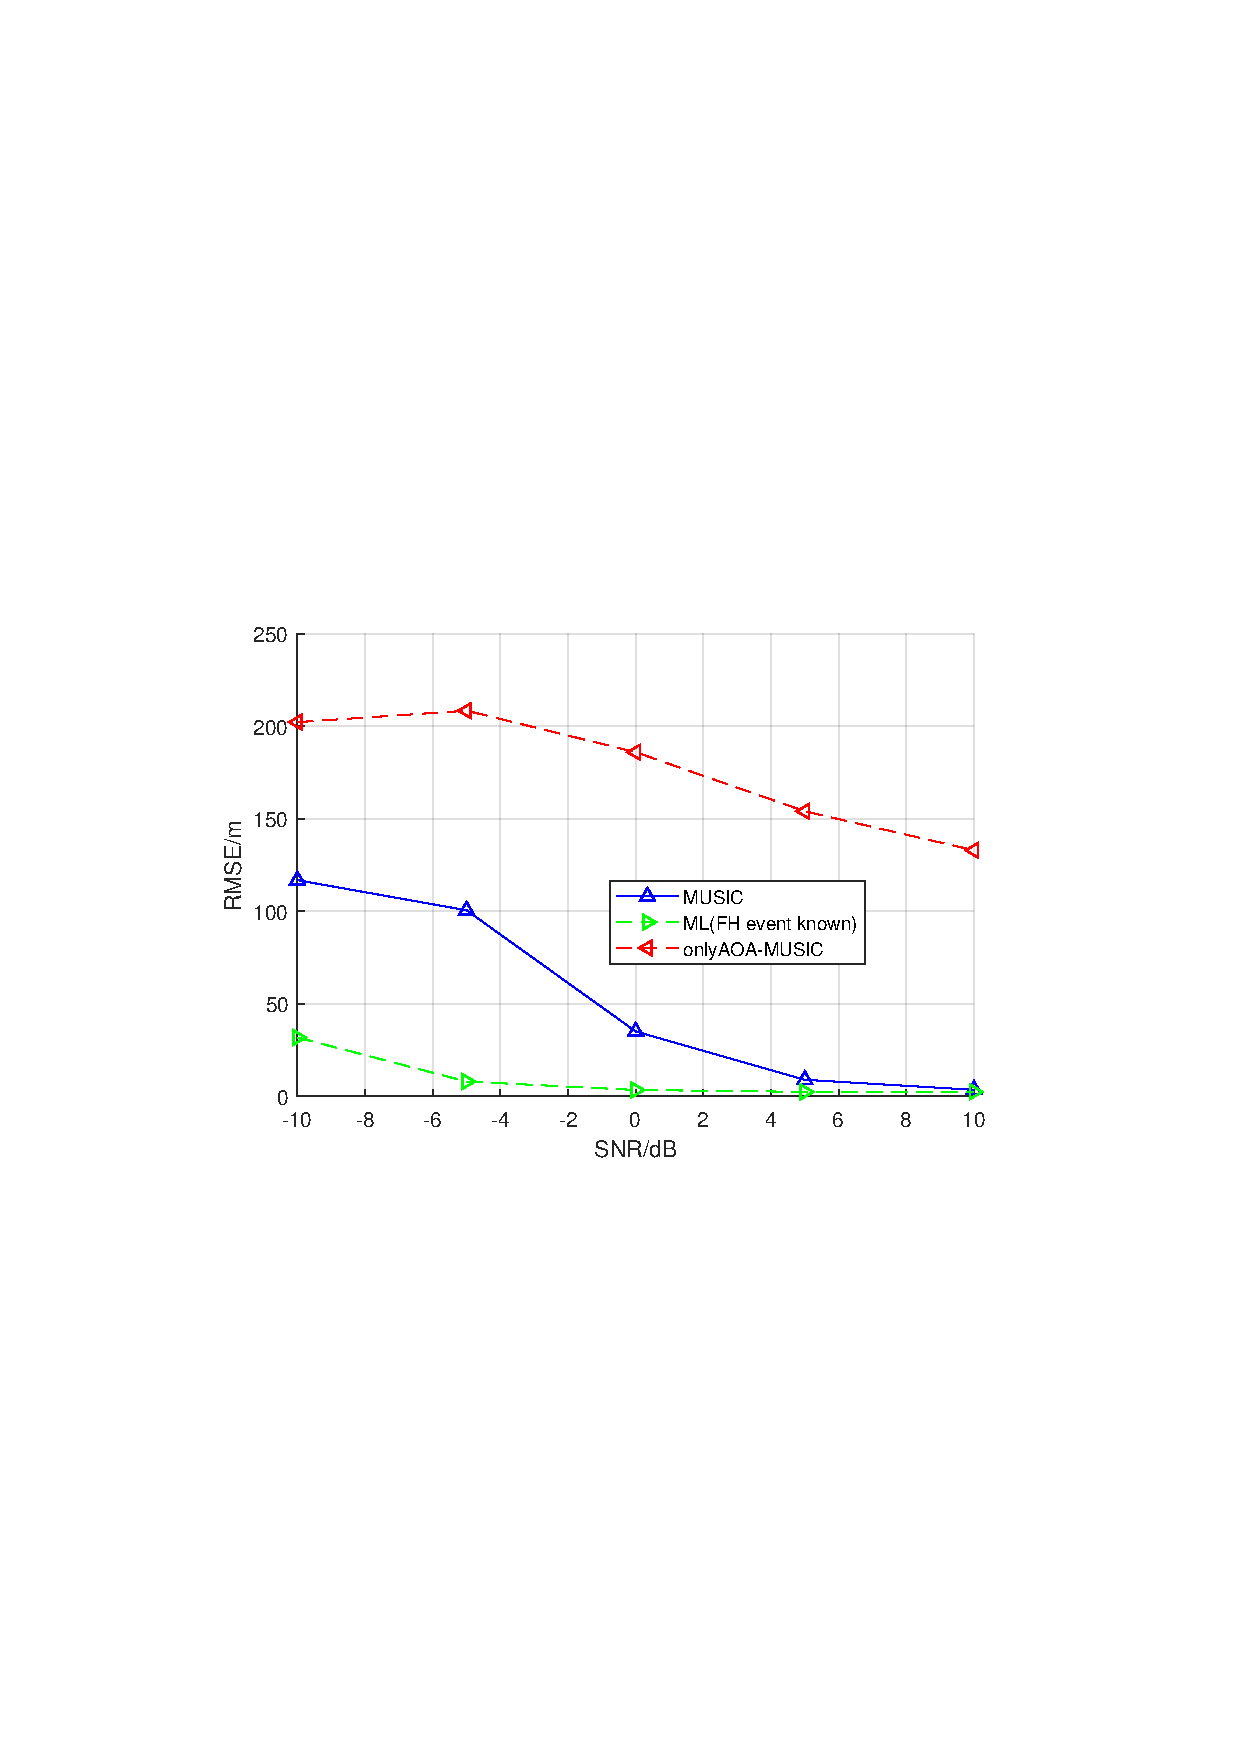
\includegraphics[width=0.48\textwidth]{figures/simu_vsSNR.pdf}}
	\caption{the accuracy of estimators vs SNR}\label{fig:1}
\end{figure}


In experiments, the $N_r=4$ receivers located at $(0,0)$km, $(0,1)$km, $(1,1)$km and $(1,0)$km respectively, each of which equipped with an uniform circle array (UCA) of $M=8$ elements, intercept $Q=2$ FH signals. 
The hopping range of the FH signals is $2$MHz, the hopping interval is $62.5$kHz (so the number of DFT points can be $K=32$), the hopping rate is $1000$hops/s and the central frequency is $400$MHz. 
The number of observation sections $L=1200$ which corresponds to the length of observation $20$ms.
The SNR is defined as SNR$=\vert\bar{u}_q(k,l)\vert^2/\sigma^2$, which is the ratio of the power of the received signal to the noise power at FH frequency. 
We use the root mean square of error (RMSE) to describe the statistic performance of the estimators.

In the first experiment, we put the two emitters at $(300,500)$m and $(700,500)$m and change the SNR between $(-10,10)$dB.
The figure \ref{fig:1} shows the RMSE (for the first emitter) of the AOA based estimator, the ML estimator ($E_{\kappa_1\dots\kappa_Q}$ known) and the proposed estimator vary with SNR. 
It can be seen that the ML and the proposed estimators outperform the AOA based estimator because the later only utilized the location information in space domain.
The performance of the proposed estimator converges to that of ML estimator which is the performance bound. That is, the proposed estimator has the asymptotic optimal performance 
since the idle frequencies can be identified perfectly at high SNR.

\begin{figure}[!t] 
	\centerline{\includegraphics[width=0.48\textwidth]{figures/MUSIC谱.pdf}}
	\caption{the proposed high resolution location spectrum (SNR=$10$dB, the blue circle denotes the real emitter locations and the red cross denotes the location estimations, the same below.)}\label{fig:2}
\end{figure}

\begin{figure}[!t] 
	\centerline{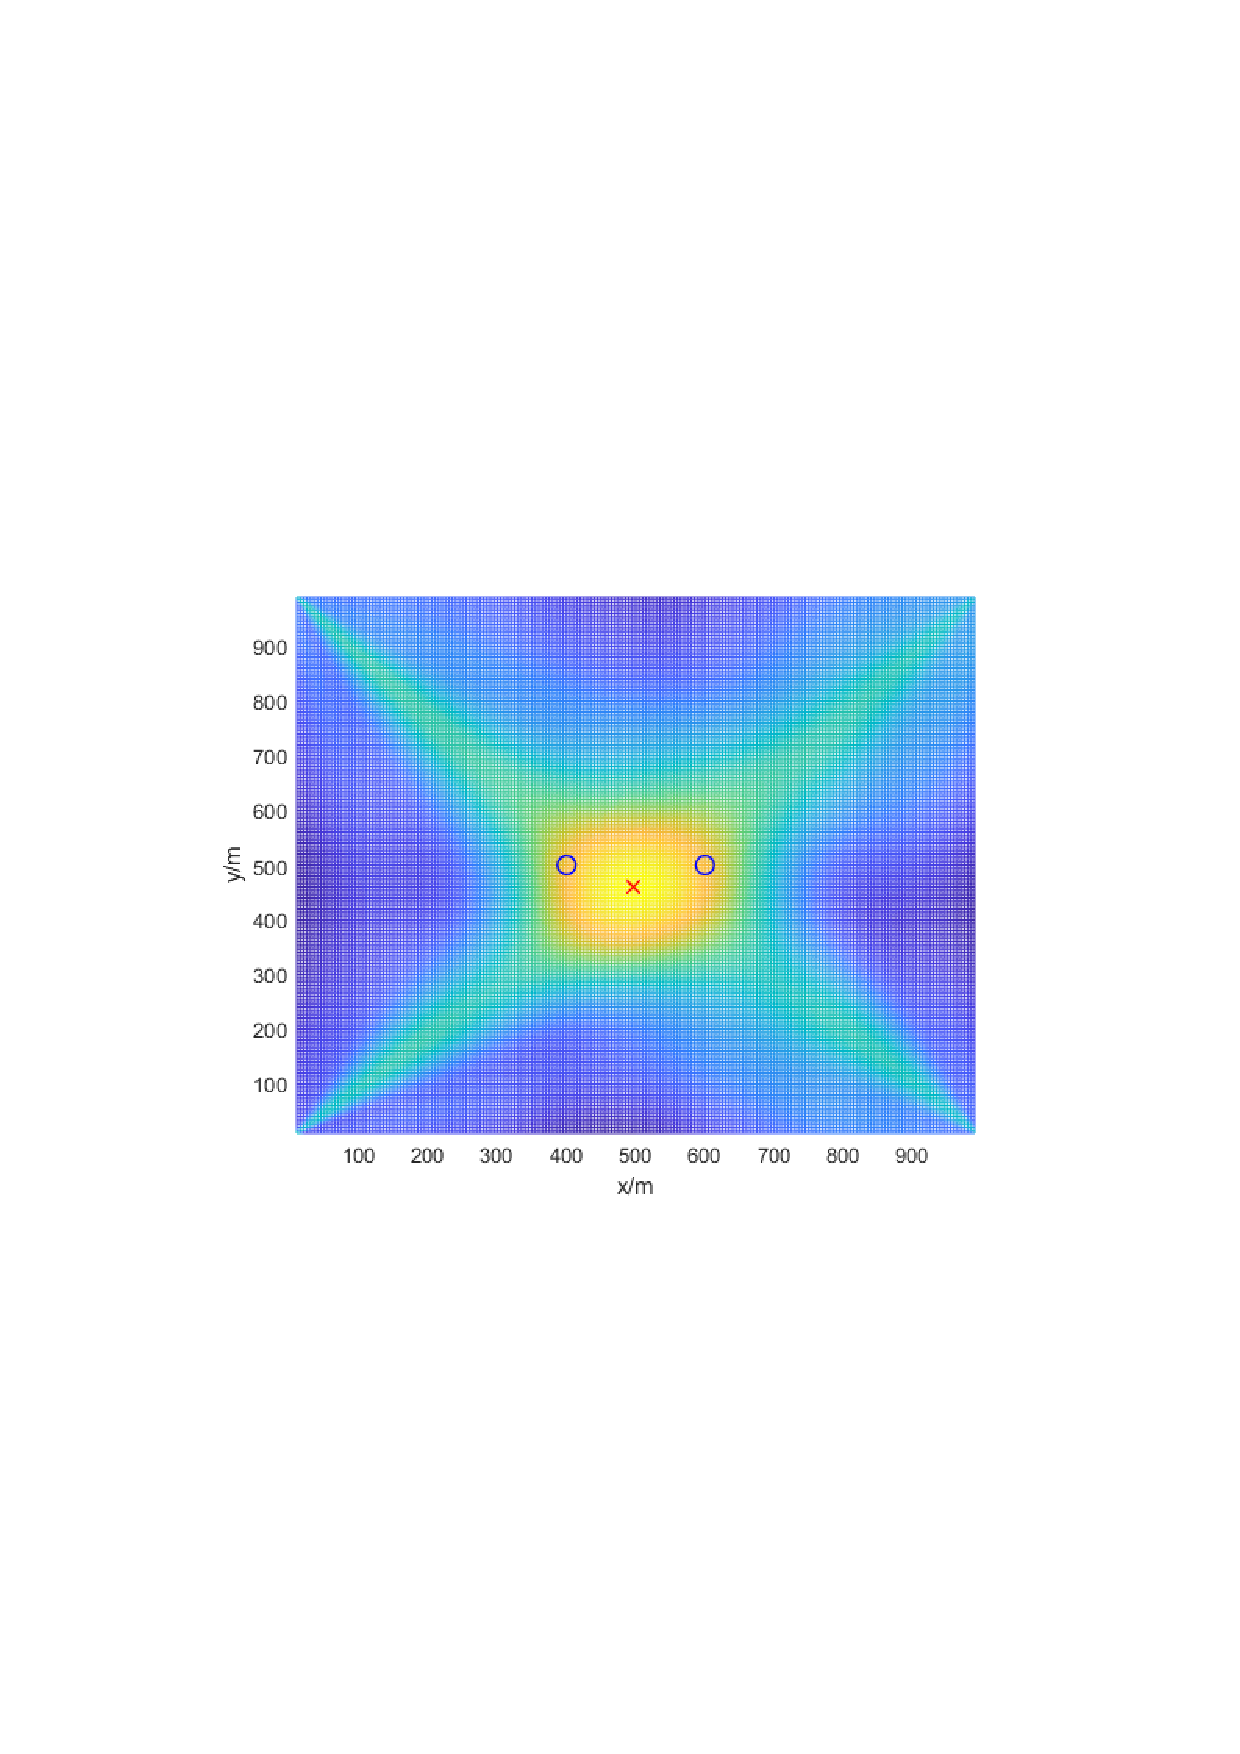
\includegraphics[width=0.48\textwidth]{figures/SML位置谱.pdf}}
	\caption{the AOA based MUSIC location spectrum}\label{fig:3}
\end{figure}

In the second experiment, we fix the SNR=$10$dB and consider two neighboring emitters at $(400,500)$m and $(600,500)$m to verify the high resolution of the proposed MUSIC based estimator. 
The figures \ref{fig:2} and \ref{fig:3} demonstrates the proposed high resolution location spectrum and the AOA based MUSIC location spectrum. It can be seen that there are two sharp peaks at the real emitter locations in the proposed location spectrum 
while there are only one wide main lobe the AOA based MUSIC location spectrum.

% By the figure \ref{fig:4}, it is noted that the RMSE of coherent estimators increase with the clock difference while that of incoherent estimators stay constant, 
% which indicates that the efficiency of coherent integration decreases because of the clock differences. Note that the coherent integration becomes noneffective (the RMSE of coherent integration stay constant) when $\sigma_t\geq 1\mu \text{s}$.

% The figure \ref{fig:2} demonstrates the ratio of $RMSE\leq1$km results to all $500$ Monte Carlo simulation results varies with SNR, which describes the stability of those estimators. 
% It can be seen that the coherent estimators (the red circle lines) outperform the incoherent ones (the blue circle lines) in synchronous scenario.
% While the performance of the coherent estimators can not be improved as SNR increasing in asynchronous scenario (the red 'x' lines), which indicates that the clock difference is more powerful to decrease the efficiency of coherent integration than noise does.
% The coherent estimators even become noneffective when the clock differences reach $1\mu\text{s}$s in the first experiment. Hence, it is necessary to use the incoherent approach in asynchronous scenario.
% We can also see the performance of incoherent estimators both in synchronous and asynchronous scenarios are similar, which indicates that incoherent estimators won't be affected by clock differences.

% By the figure \ref{fig:1} and figure \ref{fig:2}, the improvement of both coherent and incoherent original estimators are presented. The refined estimators further suppress the noise to increase the processing gain.
% The figure \ref{fig:3} shows the precision rate $\eta$ of estimating the FH pattern, which is defined as $\eta \triangleq 1-P_{fa}+P_d$ where the $P_{fa},P_d$ is false alarm and detection probabilities respectively.  
% It can be seen that the coherent approach attains higher precision rate and reaches the perfect point ($100\%$) at lower SNR.

\section{Conclusion}
\label{sec:conclusion}
In this paper, we build a data model to describe location information of multiple FH emitters both in space and frequency domain. Based on the data model, a MUSIC based algorithm is proposed to identify the idle frequencies and estimate the emitter locations simultaneously.
The proposed estimator outperforms the AOA based methods since the former integrates the location information both in space and frequency domain and the noise at idle frequencies are identified and removed.
The simulation results indicate that the proposed estimator outperforms the AOA based estimator both in the aspects of accuracy and resolution and attains asymptotic optimal performance. 

%\section*{Acknowledgment}
%The authors would like to thank...
\newpage
\bibliographystyle{unsrt}

\bibliography{refs}
\balance


\end{document}


